% ==============================================================================
% LAB 167
% MÄTNING PÅ ELEKTRISKA KRETSAR
% --------------------------
% Last updated <2015-03-10>
%
% Author:
% Jonas Sjöberg     <tel12jsg@student.hig.se>
% Oscar Wallberg    <tco13owg@student.hig.se>
%
% License:
% Creative Commons Attribution-NonCommercial-ShareAlike 4.0 International
% See LICENSE.md for full licensing information.
% ==============================================================================

% ==============================================================================
% INCLUDES AND CONFIGURATION
% ==============================================================================
\documentclass[11pt,a4paper]{article}
\usepackage[utf8]{inputenc}
\usepackage[swedish]{babel} % För svensk innehållsförteckning
\usepackage{siunitx} % (För dokumentation, kör i terminalen; texdoc siunitx)
\usepackage{amssymb}
\usepackage{amsmath}
\usepackage{amsfonts}
\usepackage{graphicx}
\usepackage{booktabs}
\usepackage{longtable} % Tables span across pages
\usepackage{microtype}
\usepackage{gensymb}
%\usepackage{tabto}
\usepackage{units}

\setlength\parindent{0pt} % Removes all indentation from paragraphs

% ==============================================================================
% DOCUMENT METADATA
% ==============================================================================
\title{EE466 \\ Lab 167 \\ Mätning på elektriska kretsar}

\author{\\
  Jonas Sjöberg\\
  Högskolan i Gävle,\\
  Elektronikingenjörsprogrammet,\\
  \texttt{tel12jsg@student.hig.se}\\
  \\
  Oscar Wallberg\\
  Högskolan i Gävle,\\
  Dataingenjörsprogrammet,\\
  \texttt{tco13owg@student.hig.se}\\}

\date{}
% ==============================================================================
\begin{document}
% ==============================================================================
\maketitle

\begin{center}
    \begin{tabular}{l r}
        Labb utförd: & ? Februari 2015 \\
        Instruktör: & Efrain Zenteno
    \end{tabular}
\end{center}

% ==============================================================================
% ABSTRACT
% ==============================================================================
\begin{abstract}
    Syftet med laborationen är att praktiskt pröva några av de grundläggande
    sambanden och satserna i likströmsläran, samt att förstå enkla
    växelströmskretsar. Dessutom bör studenten efter genomförd laboration
    översiktligt förstå universalinstrumentets och oscilloskopets principiella
    funktionssätt, samt kunna tillämpa hanteringen av dessa instrument i
    mätning på elektriska kretsar.
\end{abstract}

\newpage

{
    %\hypersetup{linkcolor=black}
    \setcounter{tocdepth}{3}
    \tableofcontents
}

\newpage

% ==============================================================================
% SECTION: INTRODUKTION
% ==============================================================================
\section{Introduktion}\label{setup}
% ==============================================================================
% TODO: Allmän introduktion.


% ==============================================================================
% SECTION: 1 MÄTNING PÅ SERIESKRETS
% ==============================================================================
\section{Mätning på seriekrets}\label{}
% ==============================================================================
% TODO: Kopplingsschema.
Seriekretsen enligt figur \ref{fig:1-mm-schem} kopplades upp. 5 \si{\volt} valdes för spänningskällan.
\begin{figure}[htbp]
    \centering
        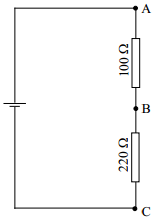
\includegraphics[scale=0.7]{misc/krets1.png}
    \caption{Seriekrets}
    \label{fig:1-mm-schem}
\end{figure}
\subsection{Mätresultat}\label{}
% ------------------------------------------------------------------------------
% TODO: + Spänningarna mellan AB, BC och AC.
Resistensen mellan A och B, $R_1$, mättes upp till $100.561 \ohm$ och mellan B och C, $R_2$, mättes $217.78 \ohm$ upp. Följande spänningar mättes därefter upp:
\begin{math}
U_{AB} = 1.58 \si{\volt}\\
U_{BC} = 3.41 \si{\volt}\\
U_{AC} = 4.999 \si{\volt}
\end{math}
\subsection{Kommentar}\label{}
% ------------------------------------------------------------------------------
% TODO: Kommentera utgående från Kirchhoffs 2:a lag.
%       Kommentera utgående från spänningsdelningslagen.
Spänningsdelningslagen ger:\\[+2mm]
\begin{math}
U_{AB} = U\times\frac{R_{1}}{R_{1}+R_{2}}\\[+2mm]
U_{AB} = 4.999\times\frac{100.561}{100.561+217.78}\\[+2mm]
U_{AB} = 1.579\\
\\
U_{BC} = U\times\frac{R_{2}}{R_{1}+R_{2}}\\[+2mm]
U_{BC} = 4.999\times\frac{217.78}{100.561+217.78}\\[+2mm]
U_{BC} = 3.42\\
\\
U_{AC} = U\times\frac{R_{1}+R_{2}}{R_{1}+R_{2}}\\[+2mm]
U_{AC} = U = 4.999\\
\end{math}

Kirchhoff's 2:a lag:
\begin{quote}
Summan av samtliga emk:s som ingår i en sluten krets är lika med summan av potentialfallen, eller\\
\begin{math}
u_{1} + u_{2} + \ldots + u_{n} = 0\\
\text{där }u_{k} \text{ betecknar en potentialändring.}
\end{math}
\end{quote}

Enligt Kirchhoff's lag:\\
$U - U_{AB} - U_{BC} = 0$\\
$4.99 - 1.579 - 3.42 = 0$, vilket stämmer.
% ==============================================================================
% SECTION: 2 iNVERKAN AV EN PARALLELLGREN PÅ EN KRETS
% ==============================================================================
\section{Inverkan av en parallellgren på en krets}\label{}
% ==============================================================================
% TODO: Kopplingsschema.

\subsection{Mätresultat}\label{}
% ------------------------------------------------------------------------------
% TODO: Mät strömmen i punkten B samt strömmen direkt från spänningskällan.


% ==============================================================================
% SECTION: 3 MÄTNING PÅ PARALLELLKRETS
% ==============================================================================
\section{Mätning på parallellkrets}\label{}
% ==============================================================================
% TODO: Kopplingsschema.

\subsection{Mätresultat}\label{}
% ------------------------------------------------------------------------------
% TODO: Mät de markerade strömmarna

\subsection{Kommentar}\label{}
% ------------------------------------------------------------------------------
% TODO: Kommentera utgående från Kirchhoffs 1:a lag.


% ==============================================================================
% SECTION: 4 MÄTNING AV RESISTANS
% ==============================================================================
\section{Mätning av resistans}\label{}
% ==============================================================================
% TODO: Kopplingsschema.

\subsection{Mätresultat}\label{}
% ------------------------------------------------------------------------------
% TODO: Mät resistansen mellan A och B i nedanstående kretsar.

\subsection{Teoretisk beräkning}\label{}
% ------------------------------------------------------------------------------
% TODO: För varje mätning skall du verifiera resultatet med en teoretisk beräkning.

%\subsection{Kommentar}\label{}
% ------------------------------------------------------------------------------
% TODO: Kommentar på skillnader mellan mätresultat och beräkning?


% ==============================================================================
% SECTION: 5 MÄTNING AV EMK OCH INRE RESISTANS I EN TVÅPOL
% ==============================================================================
\section{Mätning av emk och inre resistans i en tvåpol}\label{measure_emk}
% ==============================================================================
Dessa mätningar görs i syfte att undersöka konceptet tvåpol och demonstrera
konceptet av att studera och räkna med reducering av komplexa nät med hjälp av
Thévenins ekvivalens.  \par En så kallad experimentplatta eller "breadboard"
används för att konstruera kretsen som illustreras i Figur \ref{fig:5-schem}.
Nätaggregatet $V_{1}$ är ett strömbegränsande laboratorieaggregat HP3631A.
Spänningen $U$ mäts över dekadresistorn $R_{3}$ med bänkmultimetern $M_{2}$, en
HP34401A.  Strömmen $I$ mäts genom att den handhållna multimetern Tenma 72-2050
kopplas mellan punkten $A$ och $R_{3}$.  \par Källan som driver spänningen
$V_{AB}$ utgörs av $V_{1}$, $R_{1}$ och $R_{2}$.  \par Lasten som är ansluten
till utgången utgörs av dekadresistorn $R_{3}$.  Resistansen hos multimetern
$M_{2}$ parallellkopplas med $R_{3}$ och påverkar således kretsen på ett
oönskat sätt. Om man antar att $M_{2}$ har en inre resistans på
\unit[10]{\si{\Mohm}} förändras lastens effektiva resistans. Förändringen är
försumbar då $R_{3}$ har ett lågt värde men felvärdet blir klart påtagligt vid
högre resistansvärden.  Felvärdet kan beräknas med Ekvation \ref{eq:err1} som
vid en högre resistans enligt \ref{eq:err2} blir 0,09\%, vilket klart påverkar
mätresultatet.  Men eftersom den maximala resistansen som används är
\unit[100]{\si{\kohm}} så kan belastning från multimetern förbises.
\par Utan belastning är spänningen vid tvåpolens "utgång",
$V_{AB}$ = \unit[7.16]{\si{\volt}}.
\par Med $R_{3}$ ställd på sin maximala resistans är spänningen oförändrad.
När värdet hos $R_{3}$ sänks börjar spänningen vid tvåpolens utgång också att
sjunka.
\par Halva tomgångsspänningen $\frac{V_{AB}}{2} = \unit[3.58]{\si{\volt}}$
avläses vid en last av $R_{3}$ = \unit[341]{\si{\ohm}}.  Strömmen genom lasten
är då $I = \unit[10.531]{\si{\mA}}$.

% Obelastad polspänning  Vab = 7.16V


% Förändring i procent;
% fel(%) = [(uppmätt - förväntat) / förväntat] * 100
% (((1/((1/x)+(1/(10e6))))-x)/x)*100
\begin{equation}\label{eq:err1}
\text{Felvärde}(\si{\percent}) =
\frac{\text{Uppmätt värde} - \text{Förväntat värde}}{\text{Förväntat värde}} \times 100
\end{equation}

Vid en resistans på t.ex. \unit[1]{\si{\Mohm}} blir felvärdet enligt Ekvation
\ref{eq:err2}.  \par Ett felvärde på 0,09\% är utgör ett signifikant mätfel. I
det här fallet är lastresistansen som effektivt parallellkopplas med
multimetern mycket lägre än \unit[1]{\si{\Mohm}} och mätfelet blir inte fullt
så allvarligt.

\begin{align}
\text{Felvärde }{R}_{last}(\si{\percent}) &= \frac{(\frac{1}{\frac{1}{R_{3}}+\frac{1}{R{M_{2}}}}) - R_{3}}{R_{3}} \times 100 \label{eq:err2}\\
&= \frac{(\frac{1}{\frac{1}{\unit[1]{\si{\Mohm}}}+\frac{1}{\unit[10]{\si{\Mohm}}}}) - \unit[1]{\si{\Mohm}}}{\unit[1]{\si{\Mohm}}} \times 100\\
&= 0,09 \%
\end{align}



\begin{figure}
\centering
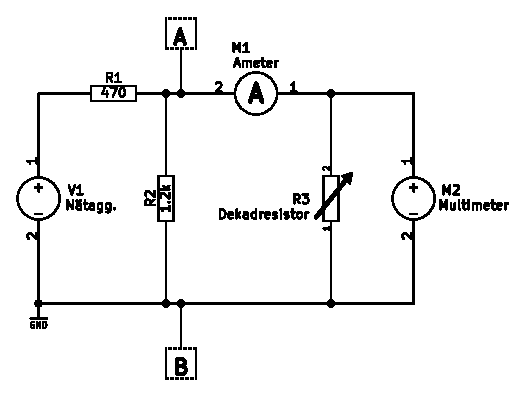
\includegraphics[width=0.7\linewidth]{img/5-schem}
\caption[Kopplingsschema för mätning av tvåpol.]
{Koppling vid mätning av EMK och inre resistans i en tvåpol.}
\label{fig:5-schem}
\end{figure}

\pagebreak

\subsection{Teoretisk härledning med Thévenins teorem}
% ------------------------------------------------------------------------------
Kretsen som levererar spänningen ritas om till den i Figur
\ref{fig:5-thevenin-schem}.

\begin{figure}
    \centering
    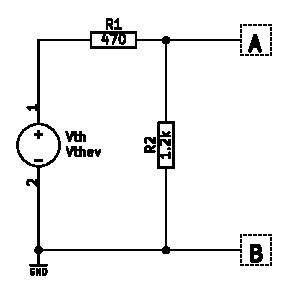
\includegraphics[width=0.4\linewidth]{img/5-thevenin-schem}
    \caption[Théveninekvivalens]
    {Den obelastade kretsen som utgör källpolspänningen}
    \label{fig:5-thevenin-schem}
\end{figure}

Den obelastade "tomgångsspänningen" mellan punkterna A och B, $V_{AB}$ beräknas
enligt Ekv. \ref{eq:thev1}.
% 10*(1,2e3/(470+1,2e3)) = 7,18562874251497005988
\begin{equation}\label{eq:thev1}
\begin{split}
V_{AB} = V_{th} \times \frac{R_2}{R_1 + R_2}\\
V_{AB} = \unit[10]{\si{\volt}} \times \frac{\unit[1.2]{\si{\kohm}}}{\unit[470]{\si{\ohm}}+ \unit[1.2]{\si{\kohm}}}\\
V_{AB} = \unit[10]{\si{\volt}} \times \frac{\num{1.2e3}}{\num{470}+\num{1.2e3}}\\
V_{AB} = \unit[7,185]{\si{\volt}}
\end{split}
\end{equation}

Den inre resistansen beräknas genom att kortsluta spänningskällan.
Kretsen blir då den i Figur \ref{fig:5-thevenin-schem2}.

\begin{figure}
    \centering
    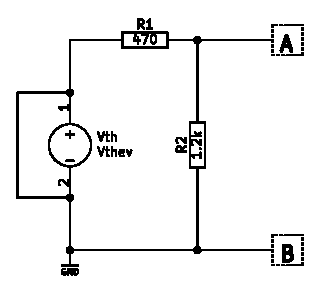
\includegraphics[width=0.4\linewidth]{img/5-thevenin-schem2}
    \caption[Beräkning av Théveninekvivalens]
    {Spänningskälla kortsluten för att hitta inre resistans}
    \label{fig:5-thevenin-schem2}
\end{figure}

Den inre resistansen utgörs av parallellkopplingen $R_{1}$ och $R_{2}$ och
beräknas enligt Ekv. \ref{eq:thev2}.
% (470*1200)/(470+1200) = 337,72455089820359281437
\begin{equation}\label{eq:thev2}
\begin{split}
R_{th} = \frac{1}{\frac{1}{R_{1}} + \frac{1}{R_{2}}}\\
R_{th} = \frac{1}{\frac{1}{\unit[470]{\si{\ohm}}} + \frac{1}{\unit[1.2]{\si{\kohm}}}}\\
R_{th} = \unit[337,72]{\si{\ohm}}
\end{split}
\end{equation}

De teoretiska värdena för Théveninekvivalensen i \ref{eq:thev3} används i Figur
\ref{fig:5-thevenin-schem3} som har ett beteende ekvivalent med den
ursprungliga tvåpolen.

\begin{align}\label{eq:thev3}
V_{AB} &= \unit[7,185]{\si{\volt}}\\
R_{th} &= \unit[337,72]{\si{\ohm}}
\end{align}

\begin{figure}
    \centering
    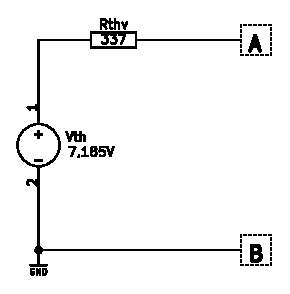
\includegraphics[width=0.4\linewidth]{img/5-thevenin-schem3}
    \caption[Beräkning av Théveninekvivalens]
    {Fullständig ekvivalent krets}
    \label{fig:5-thevenin-schem3}
\end{figure}

\pagebreak

% ==============================================================================
% SECTION: 6 KARAKTERISTIK HOS EN LYSDIOD
% ==============================================================================
\section{Karakteristik hos en lysdiod}\label{}
% ==============================================================================
% TODO: Rita grafen I=f(U)! Kommentera!

\begin{longtable}[c]{@{}ccc@{}}
    \toprule\addlinespace
    \begin{tabular}{ll}$R_{3}$
    \end{tabular} & \begin{tabular}{ll}$I_{M1}$
\end{tabular} & \begin{tabular}{ll}$V_{M2}$
\end{tabular}
\\\addlinespace
\midrule\endhead
\unit[500]{\si{\ohm}} & \unit[16.38]{\si{\unit{\mA}}} & \unit[1.78]{\si{\volt}}
\\\addlinespace
\unit[600]{\si{\ohm}} & \unit[13.66]{\si{\unit{\mA}}} & \unit[1.766]{\si{\volt}}
\\\addlinespace
\unit[700]{\si{\ohm}} & \unit[11.725]{\si{\unit{\mA}}} & \unit[1.755]{\si{\volt}}
\\\addlinespace
\unit[800]{\si{\ohm}} & \unit[10.269]{\si{\unit{\mA}}} & \unit[1.744]{\si{\volt}}
\\\addlinespace
\unit[900]{\si{\ohm}} & \unit[9.1342]{\si{\unit{\mA}}} & \unit[1.737]{\si{\volt}}
\\\addlinespace
\unit[1]{\si{\kohm}} & \unit[8.260]{\si{\unit{\mA}}} & \unit[1.730]{\si{\volt}}
\\\addlinespace
\unit[2]{\si{\kohm}} & \unit[3.3319]{\si{\unit{\mA}}} & \unit[1.685]{\si{\volt}}
\\\addlinespace
\unit[3]{\si{\kohm}} & \unit[2.3805]{\si{\unit{\mA}}} & \unit[1.671]{\si{\volt}}
\\\addlinespace
\unit[4]{\si{\kohm}} & \unit[1.8525]{\si{\unit{\mA}}} & \unit[1.662]{\si{\volt}}
\\\addlinespace
\unit[5]{\si{\kohm}} & \unit[1.5176]{\si{\unit{\mA}}} & \unit[1.655]{\si{\volt}}
\\\addlinespace
\unit[6]{\si{\kohm}} & \unit[1.2858]{\si{\unit{\mA}}} & \unit[1.648]{\si{\volt}}
\\\addlinespace
\unit[7]{\si{\kohm}} & \unit[1.1159]{\si{\unit{\mA}}} & \unit[1.643]{\si{\volt}}
\\\addlinespace
\unit[8]{\si{\kohm}} & \unit[985.6]{\si{\unit{\uA}}} & \unit[1.637]{\si{\volt}}
\\\addlinespace
\unit[9]{\si{\kohm}} & \unit[882.5]{\si{\unit{\uA}}} & \unit[1.6304]{\si{\volt}}
\\\addlinespace
\unit[10]{\si{\kohm}} & \unit[799.2]{\si{\unit{\uA}}} & \unit[1.630]{\si{\volt}}
\\\addlinespace
\unit[20]{\si{\kohm}} & \unit[408.7]{\si{\unit{\uA}}} & \unit[1.605]{\si{\volt}}
\\\addlinespace
\unit[30]{\si{\kohm}} & \unit[275.3]{\si{\unit{\uA}}} & \unit[1.590]{\si{\volt}}
\\\addlinespace
\unit[40]{\si{\kohm}} & \unit[2077]{\si{\unit{\uA}}} & \unit[1.578]{\si{\volt}}
\\\addlinespace
\unit[50]{\si{\kohm}} & \unit[1667]{\si{\unit{\uA}}} & \unit[1.569]{\si{\volt}}
\\\addlinespace
\unit[60]{\si{\kohm}} & \unit[139.2]{\si{\unit{\uA}}} & \unit[1.567]{\si{\volt}}
\\\addlinespace
\unit[70]{\si{\kohm}} & \unit[496.]{\si{\unit{\uA}}} & \unit[1.556]{\si{\volt}}
\\\addlinespace
\unit[80]{\si{\kohm}} & \unit[104.8]{\si{\unit{\uA}}} & \unit[1.55]{\si{\volt}}
\\\addlinespace
\unit[90]{\si{\kohm}} & \unit[93.3]{\si{\unit{\uA}}} & \unit[1.545]{\si{\volt}}
\\\addlinespace
\unit[100]{\si{\kohm}} & \unit[84.0]{\si{\unit{\uA}}} & \unit[1.541]{\si{\volt}}
\\\addlinespace
\bottomrule
\addlinespace
\caption[]{Mätresultat för kretsen i Figur \ref{fig:5-schem}.}
\label{emktable}
\end{longtable}

% ==============================================================================
% SECTION: 7 MÄTNING AV VÄXELSPÄNNING MED UNIVERSALINSTRUMENT OCH OSCILLOSKOP
% ==============================================================================
\section{Mätning av växelspänning med universalinstrument och oscilloskop}\label{}
% ==============================================================================
% TODO


% ==============================================================================
% SECTION: 8 STUDIUM AV FREKVENSGÅNG I EN REAKTIV KRETS
% ==============================================================================
\section{Studium av frekvensgång i en reaktiv krets}\label{}
% ==============================================================================
% TODO: Kopplingsschema.

\subsection{Mätresultat}\label{}
% ------------------------------------------------------------------------------
% TODO: + Gör upp en tabell som för varje frekvens anger
%         - tongeneratorns signalamplitud,
%         - amplituden hos spänningen över den studerade kondensatorn
%         - kvoten mellan den senare amplituden och den tidigare
%         - samt om fasförskjutning förekommer.

\subsection{Teoretisk beräkning}\label{}
% ------------------------------------------------------------------------------
% TODO: Kontrollera dina resultat genom att utnyttja följande formel:

\subsection{Kommentar}\label{}
% ------------------------------------------------------------------------------
% TODO:


% ==============================================================================
% SECTION: 9 MÄTNING AV FASFÖRSKJUTNING I EN REAKTIV KRETS
% ==============================================================================
\section{Mätning av fasförskjutning i en reaktiv krets}\label{}
% ==============================================================================
% TODO: Kopplingsschema.
%       Samma koppling som förra uppgiften, kanske överflödigt att upprepa?

\subsection{Mätresultat}\label{}
% ------------------------------------------------------------------------------
% TODO:

\subsection{Teoretisk beräkning}\label{}
% ------------------------------------------------------------------------------
% TODO: Kontrollera dina resultat genom att utnyttja följande formel:

\subsection{Kommentar}\label{}
% ------------------------------------------------------------------------------
% TODO: Kommentera resultatet


% ==============================================================================
% SECTION: 10 MÄTNING AV RESONANSFREKVENS
% ==============================================================================
\section{Mätning av resonansfrekvens}\label{}
% ==============================================================================
% TODO: Kopplingsschema.

\subsection{Mätresultat}\label{}
% ------------------------------------------------------------------------------
% TODO: Notera resonansfrekvensen.

\subsection{Kommentar}\label{}
% ------------------------------------------------------------------------------
% TODO: + Kommentera följande:
%          - Förekommer fasförskjutning mellan uTG och uR vid denna frekvens?
%          - Ändrar fasen sig om du varierar frekvensen kring den
%            uppmätta resonansfrekvensen?  I så fall hur?
%          - Om laboration 61 har gjorts, jämför resultatet med de uppmätta
%            värderna.  Stämmer de överens om inte, varför?


% ==============================================================================
% SECTION: RESULTAT
% ==============================================================================
\section{Resultat}\label{setup}
% ==============================================================================
% TODO: Övergripande resultat/sammanfattning/kommentar på HELA labben.

\newpage

% ==============================================================================
% SECTION: REFERENSER
% ==============================================================================
\section{Referenser}\label{refs}
% ==============================================================================
%TODO: Referenser.

%\subsection{www}\label{interwebs}
% ------------------------------------------------------------------------------

%\subsection{Trycksaker}\label{literature} %???
% ------------------------------------------------------------------------------

%\subsection{Källkod}\label{sourcefiles}
% ------------------------------------------------------------------------------

% ==============================================================================
\end{document}
% ==============================================================================
